\documentclass{article}
\usepackage[utf8]{inputenc}
\usepackage{fancyhdr}
\usepackage{lastpage}

\usepackage{float}

\usepackage{hyperref}
\usepackage{tikz} 
\usetikzlibrary{shapes,arrows}

\usepackage[margin=3cm]{geometry}
\usepackage{amssymb}
\usepackage{amsthm}
\usepackage{amsmath}
\usepackage{pgfgantt}
\graphicspath{{img/}{../img/}}

\usepackage{pgfplots, pgfplotstable}
\pgfplotsset{compat=newest}
\usepgfplotslibrary{colormaps}
\usepackage{xstring}
\usepackage{caption}

\usepackage{subcaption}



\usepackage{listings}
\lstset{
  basicstyle=\ttfamily,
  columns=fullflexible,
  frame=single,
  breaklines=true,
  postbreak=\mbox{\textcolor{red}{$\hookrightarrow$}\space},
}

\pagestyle{fancy}
\fancyhf{}
\begin{document}

\section{Context}

\section{Quadcopter Model}

For the physics model, the coordinate space is referred to using \emph{local tangent plane coordinates}, namely that $z$ is east, $x$ is north and $y$ is up. The principal axes of movement are \emph{pitch}, along the transverse ($z$) axis, \emph{roll}, along the longitudinal ($x$) axis, and \emph{yaw}, along the vertical ($y$) axis.

A UAV can be modelled as a rigid body with mass $m$, on Earth. As such, gravity acts on the agent at $9.81\frac{m}{s^2}$. The drag coefficient is estimated at $0.975$ considering the mass of the body \cite{Hattenberger}.

The dimensions and chracteristics of the agent have been determined using both realistic averages \cite{Figliozzi} and estimations. These can be seen in Fig. \ref{fig:dimensions}.

\begin{figure}[H]
    \centering
    \begin{tabular}{| c | c |} 
    \hline
    Parameter & Value \\ 
    \hline
    Mass, $m$ & 10 kg \\
    \hline
    Length, $l$ & 0.7 m \\
    \hline
    Width, $w$ & 0.7 m \\
    \hline
    Height, $h$ & 0.25 m \\
    \hline
    Propeller Area, $A$ & 0.16 m$^2$ \\
    \hline
    Distance To Propeller Centre, $d$ & 0.5 m \\
    \hline
    Drag Coefficient, $C_d$ & 0.975 \\
    \hline
    \end{tabular}
    \caption{Dimensions of the Agent}
    \label{fig:dimensions}
\end{figure}

The agent is modelled as a quadcopter, with four propellers. These can be independently controlled to affect the movement of the agent.

\begin{figure}[H]
    \centering
    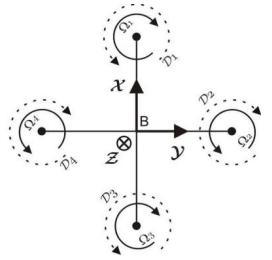
\includegraphics[height=80px]{prop.png}
    \hspace{1cm}
    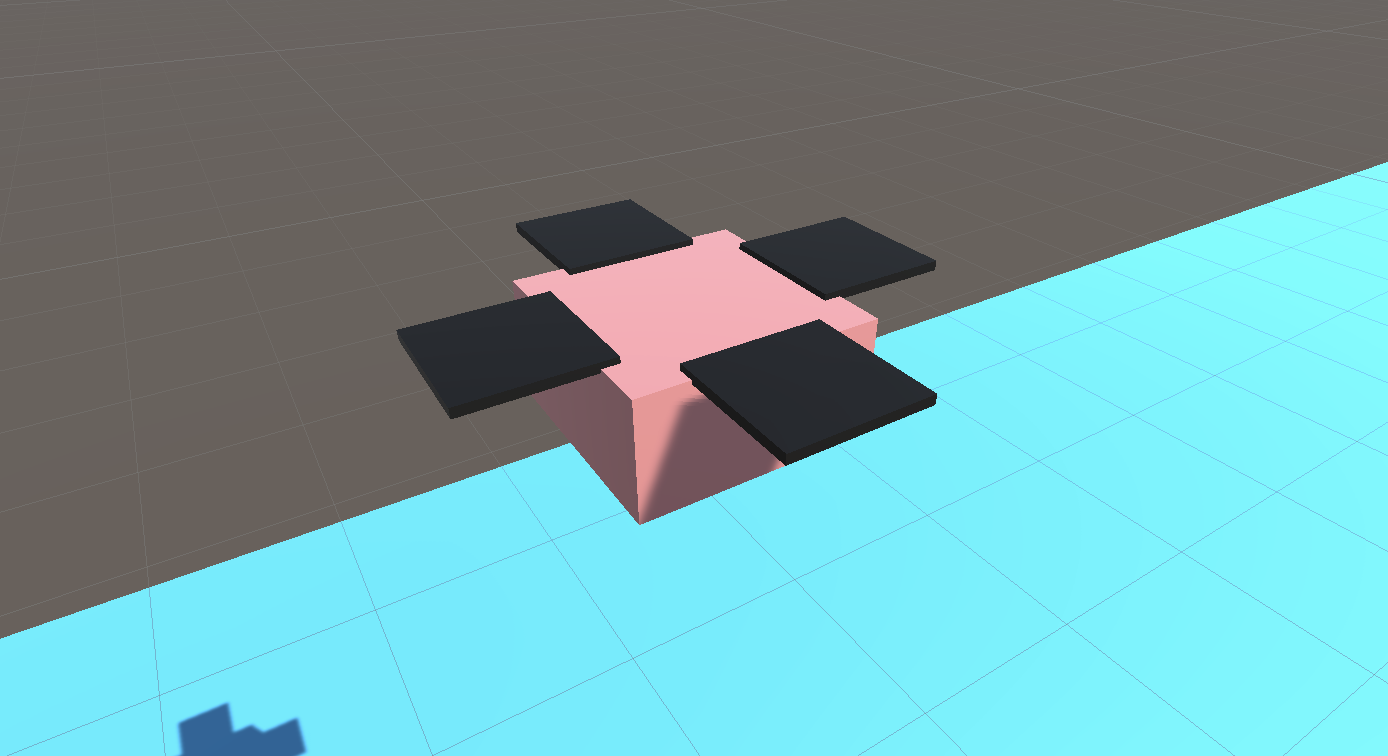
\includegraphics[height=80px]{drone-unity.png}
    \caption{Propeller Diagram \& Simulated Agent}
\end{figure}

For this investigation, a quadcopter was chosen as the type of agent, rather than a fixed-wing aircraft, due to increased maneouverability, simplicity when considering autonomous flight and simplicity in takeoff and landing procedures \cite{Thamm}.

There are four elements of control for an agent:
\begin{itemize}
    \item Roll angle (in radians), $\psi$
    \item Pitch angle (in radians), $\theta$
    \item Yaw rate (in $\frac{rad}{s}$), $\phi$
    \item Vertical thrust (in Newtons), $T$
\end{itemize}

For simplicity, these can be solely controlled by combinations of propeller thrust levels. 

A base thrust level, $T_b$, can be defined, which is the minimum thrust level required to maintain a stable hover. This is the thrust level required to counteract gravity, so $T_b = mg$. For each control operation, $T_b$ can be augmented by a thrust level, $T_{add}$, such that $|T_{add}| < T_b$, which is the additional thrust required to perform the operation.

As such, the control parameters can be operated by the following eight combinations of thrust levels for each propeller, with a high thrust level $T_{add} > 0$ and a low thrust level $T_{add} < 0$:


\begin{figure}[H]
    \begin{center}
    \begin{tabular}{| c | c | c |} 
    \hline
    Operation & High Thrust & Low Thrust \\ 
    \hline
    Positive Roll, $\psi_+$ & $D_4$ & $D_2$ \\
    \hline
    Negative Roll, $\psi_-$ & $D_2$ & $D_4$ \\
    \hline
    Positive Pitch, $\theta_+$ & $D_3$ & $D_1$ \\
    \hline
    Negative Pitch, $\theta_-$ & $D_1$ & $D_3$ \\
    \hline
    Positive Thrust, $T_+$ & $D_1, D_2, D_3, D_4$ & none \\
    \hline
    Negative Thrust, $T_-$ & none & $D_1, D_2, D_3, D_4$ \\
    \hline
    \end{tabular}
    \end{center}
    \caption{Control Operations and Thrust Levels}
    \label{fig:control}
\end{figure}


It is noted that yaw is omitted from Fig. \ref{fig:control}. For the purposes of the simulation, the propellers do not rotate. This lends itself to needing a workaround for simulating yaw. In \emph{Unity}'s physics engine, the rotation of opposite propellers can be simulated by applying forces along the $x$ and $z$ axes. As such, yaw is simulated according to the table below:

\begin{figure}[H]
    \begin{center}
    \begin{tabular}{| c | c | c |} 
    \hline
    Operation & Propeller & Direction of Force (respectively) \\ 
    \hline
    Positive Yaw, $\phi_+$ & $D_1, D_2$ & $Z_-, X_-$ \\
    \hline
    Positive Yaw, $\phi_+$ & $D_3, D_4$ & $Z_+, X_+$ \\
    \hline
    Negative Yaw, $\phi_-$ & $D_1, D_2$ & $Z_+, X_+$ \\
    \hline
    Negative Yaw, $\phi_-$ & $D_3, D_4$ & $Z_-, X_+$ \\
    \hline
    \end{tabular}
    \end{center}
    \caption{Yaw Directions and Respective Forces}
    \label{fig:yaw-control}
\end{figure}

In real world physics, a couple of propellers could not provide thrust in both extremes of the same axes, as they could not switch rotation direction. Likewise, forces in adjacent propellers would not cause rotation in the same direction. However, for the purposes of simplicity within the simulation, this is ignored.

It is then possible to set some thrust constants for each control operation. An example assigment for the pitch and roll operations is seen below in Fig. \ref{fig:thrust-constants}.

\begin{figure}[H]
    \begin{center}
    \begin{tabular}{| c | c | c |} 
    \hline
    Thrust Level & Thrust ($N$) \\ 
    \hline
    High & $\frac{2m \cdot g}{4}$\\
    \hline
    Normal & $\frac{m \cdot g}{4}$\\
    \hline
    Low & $\frac{0.5m \cdot g}{4}$\\
    \hline
    \end{tabular}
    \end{center}
    \caption{Thrust Constants for a drone of mass $m$ kg}
    \label{fig:thrust-constants}
\end{figure}

\section{Stabilisation: Proportional-Integral-Derivative Controller}
\label{sec:stabilisation}

An issue arises with this implementation; the simulation becomes unstable as thrust cannot be provided in an accurate enough manner to counteract excessive rotation, notably in the roll and pitch axes. 

As such, the need for a control system becomes apparent. A PID (Proportional-Integral-Derivative) is a feedback control system, which uses the error between the current state and the desired state to calculate the control parameters.

Fig. \ref{fig:pid} shows the feedback loop of the PID controller. The error, $e(t)$, is calculated as the difference between the desired state, $r$, and the current state, $y$. The error is then fed into the three controllers. The output of each controller is then summed to produce the control variable, $u(t)$, which is then fed into the system. The system then produces the output, $y$, which is fed back into the error calculation.

\begin{figure}[H]
    \centering
    \tikzstyle{block} = [draw, fill=blue!20, rectangle, 
    minimum height=1em, minimum width=6em]
    \tikzstyle{sum} = [draw, fill=blue!20, circle, node distance=1cm]
    \tikzstyle{input} = [coordinate]
    \tikzstyle{output} = [coordinate]
    \tikzstyle{pinstyle} = [pin edge={to-,thin,black}]

    \begin{tikzpicture}[auto, node distance=2cm,>=latex']

    \node [input, name=input1] {};
    \node [sum, right of=input1] (sum) {$\Sigma$};
    \node [block, right of=sum, node distance=2.5cm] (I) {Integral};
    \node [block, above of=I, node distance=0.8cm] (P) {Proportional};
    \node [block, below of=I, node distance=0.8cm] (D) {Derivative};
    \node [sum, right of=I, node distance=2cm] (system) {$\Sigma$};
    \node [block, right of=system, node distance=2.5cm] (quad) {Quadcopter};
    \node [output, right of=quad] (output) {};

    \draw [draw,->] (input1) -- node {$r$} (sum);
    \draw [->] (sum) -- node {$e(t)$} (I);
    \draw [->] (sum) |- node {} (P.west);
    \draw [->] (sum) |- node {} (D.west);
    \draw [->] (I) -- node {} (system);
    \draw [->] (P) -| node {} (system);
    \draw [->] (D) -| node {} (system);
    \draw [->] (system) -- node {$u(t)$} (quad);
    \draw [->] (quad) -- node {$y$} (output);
    \draw [->] (quad.south) -- +(0,-1) -- +(-7.35,-1) -- node[] {-} (sum.200);
    \end{tikzpicture}
    \caption{PID Controller}
    \label{fig:pid}
\end{figure}


The PID controller is defined by three constant parameters, $K_p$, $K_i$ and $K_d$, which are the proportional, integral and derivative gains respectively. The control variable, $u(t)$, is then defined as:

$$u(t) = K_p e(t) + K_i \int_0^t e(\tau) d\tau + K_d \frac{de(t)}{dt}$$

where $e(t)$ is the error at time $t$. Considering our simulation operates in discrete time intervals (frames), this can be approximated, using the \emph{Laplace transform} as:

$$u(t) = K_p e(t) + K_i \frac{(e_t+e_{t-1})t}{2} + K_d \frac{e_t-e_{t-1}}{t}$$

Hence, a feedback loop of the entire system can be produced, taking into account different PID controllers for each control operation. This is shown in Fig. \ref{fig:pid-feedback}.

\begin{figure}[H]
    \centering
    \tikzstyle{block} = [draw, fill=blue!20, rectangle, 
    minimum height=1em, minimum width=6em]
    \tikzstyle{sum} = [draw, fill=blue!20, circle, node distance=1cm]
    \tikzstyle{input} = [coordinate]
    \tikzstyle{output} = [coordinate]
    \tikzstyle{pinstyle} = [pin edge={to-,thin,black}]

    \begin{tikzpicture}[auto, node distance=1.3cm,>=latex']

    \node [input, name=altitude] {$T$};
    \node [input, name=pitch, below of=altitude] {$\theta$};
    \node [input, name=roll, below of=pitch] {$\psi$};
    \node [input, name=yaw, below of=roll] {$\phi$};

    \node [block, right of=altitude, node distance=2.5cm] (alt) {$PID_{altitude}$};
    \node [block, right of=pitch, node distance=2.5cm] (pt) {$PID_{pitch}$};
    \node [block, right of=roll, node distance=2.5cm] (rl) {$PID_{roll}$};
    \node [block, right of=yaw, node distance=2.5cm] (yw) {$PID_{yaw}$};


    \node [input, name=guide1, right of=pt, node distance=2.5cm] {};
    \node [input, name=guide2, right of=rl, node distance=2.5cm] {};

    \node [block] (output) at ($(guide1)!0.5!(guide2)$) {Quadcopter};

    \draw [->] (altitude) -- node {$T$} (alt);
    \draw [->] (pitch) -- node {$\theta$} (pt);
    \draw [->] (roll) -- node {$\psi$} (rl);
    \draw [->] (yaw) -- node {$\phi$} (yw);

    \draw [->] (alt.east) -| +(0.2,+0.4) -- +(-2.5,+0.4) |- node[] {} (alt.170);
    \draw [->] (pt.east) -| +(0.2,+0.4) -- +(-2.5,+0.4) |- node[] {} (pt.170);
    \draw [->] (rl.east) -| +(0.2,+0.4) -- +(-2.5,+0.4) |- node[] {} (rl.170);
    \draw [->] (yw.east) -| +(0.2,+0.4) -- +(-2.5,+0.4) |- node[] {} (yw.170);

    \draw [->] (alt.east) -| node {} (output);
    \draw [->] (pt.east) -| node {} (output);
    \draw [->] (rl.east) -| node {} (output);
    \draw [->] (yw.east) -| node {} (output);

    \end{tikzpicture}
    \caption{System Model}
    \label{fig:pid-feedback}
\end{figure}

The constants are then tuned to generate expected stabilisation behaviour. As mentioned previously, each propeller has a base thrust level equal to the force required to hover, $T_b = \frac{mg}{4}$. The PID controller is then used to calculate the thrust level to be added to each propeller, $T_{add}$, in every frame of the simulation, to perform the desired operation.

Using manual tuning, the values were optimised as shown in Fig. \ref{fig:pid-tuning}

\begin{figure}[H]
    \centering
        \begin{tabular}{| c | c | c | c |} 
        \hline
        Control Operation & $K_p$ & $K_i$ & $K_d$ \\ 
        \hline
        Thrust & 6 & 5 & 2 \\
        \hline
        Pitch & 10 & 10 & 2 \\
        \hline
        Roll & 10 & 10 & 2 \\
        \hline
        Yaw & 10 & 10 & 2 \\
        \hline
        \end{tabular}
        \caption{Tuning Constants}
        \label{fig:pid-tuning}
\end{figure}

It is noted that the agent is slightly unstable at very small angles. This is negligible.

\subsection{Faults - Oscillation}

\section{Methodology}
Qual + Quant analysis!
\subsection{Problem Statements}
\subsubsection{Scenario 1: Reaching the goal is paramount}

\subsubsection{Scenario 2: Collisions are to be avoided at all costs}

\subsubsection{Scenario 3: Performing reconnaisance of an area}

\section{Autonomy}
The initial aim is to achieve position control for an agent, such that when given a current position $[x_0,y_0,z_0]$ and a goal position $[x_1,y_1,z_1]$, the agent will move to the goal position.

There are several methods for this. An agent may yaw to face the goal, then pitch towards it. In the case of this project, time-sensitive position decisions will need to be made when considering swarm dynamics and collision avoidance, so a more efficient method is required. As such, the aim will be to pitch and roll towards the position.

This can be split up into two main goals:
\begin{enumerate}
    \item Apply a force in the opposite direction when avoiding other agents.
    \item Use trigonometry to apply relative $\phi$ and $\theta$ forces, reducing these forces when closer to the goal using a separate PID position controller.
\end{enumerate}

\subsection{Agent Vision}
\label{sec:vision}
Initially, we define what an agent can `see'. We assume that an agent knows the positions of all other agents within a certain radius, $r$. This is defined as the \emph{neighbourhood radius}. This is a constant that can be tuned. We also assume that an agent can see the goal position, $[x_1,y_1,z_1]$, and its current position, $[x_0,y_0,z_0]$.

For the purposes of foreign obejcts in the simulation, namely terrain and obstacles, we will simulate the agents as having a light ranging device, namely LiDAR, which can detect the distance to the nearest object in a given direction. The \emph{Unity} physics engine has a built-in method for this, \verb|Physics.Raycast()|. This returns the distance to the nearest object in a given direction, or \verb|Infinity| if no object is detected. Whilst this is a significant abstraction of the real world implementation of a LiDAR sensor, it is sufficient for the purposes of this simulation. We go into more detail on the implementation of this in Section \ref{sec:terrain-avoidance}.

\subsection{Boids: Flocking Behaviour}

Initially, multiple agents are now introduced into the environment and are programmed to hover. We will define two constants to assist in the autonomy of the agents. First, an avoidance radius; namely, the \emph{square avoidance radius}. For the purposes of algorithmic efficiency, we compare the magnitude of a vector, squared, between agents to the defined square avoidance radius, as per \emph{Unity}'s recommendation \cite{unity}. We also specify the number of agents to generate and the spawn radius in which to generate them. Finally, we define the \emph{neighbour radius}, defined as the radius in which an agent will consider other agents as neighbours. This is used to reduce the number of calculations required for each agent, as it will only consider nearby agents.

Notably, we must also define the implementation of `applying a force $F$ to an agent' with respect to the agents' control parameters. Initially, we consider the difference between the position vector in the agent's local frame and the environment's global frame, namely, the rotation matrix that characterises the agent's orientation. The mathematics of such an operation is outside the scope of this report. In short, we can either calculate the rotation matrix, $R$, representing this change of frame and utilise a transformation matrix, such that $F_{global} = R \cdot F_{local}$, or use quarternions to represent the change of frame. \emph{Unity} has a built in method to handle this, but the source code is obfuscated. We will utilise this method, \verb|transform.InverseTransformVector()|, to calculate the force vector in the agent's local frame. This can then be split up into the constituent pitch and roll magnitudes by taking the $x$ and $z$ components respectively.

We then introduce Reynolds' principles \cite{Reynolds} to simulate some flock behaviour. The first principle, \emph{separation}\footnote{In Reynolds' original article, this is called \emph{collision avoidance}}. In practice, this is done as follows:

\begin{enumerate}
    \item For each agent, calculate the distance to each other agent within the neighbour radius.
    \item For each distance, if the magnitude of the vector is less than the square avoidance radius, add the vector to the total force vector.
    \item Divide the total force vector by the number of agents within the neighbour radius.
    \item Apply the force vector to the agent.
\end{enumerate}

To implement the second principle, \emph{alignment}, we take the heading of each agent within the neighbour radius and average them. We then apply a force in the direction of the average heading to the agent. As with the separation principle, this force is separated into pitch and roll components.

Finally, we implement the third principle, \emph{cohesion}. This is in principle, the inverse to the separation principle. Hence, this is implemented as follows:

\begin{enumerate}
    \item For each agent, find the global position of each other agent within the neighbour radius.
    \item Sum all these positions and divide them by the number of neighbours to find the average position between all neighbours.
    \item Subtract the agent's current position from the average position to find the force vector between the two.
    \item Apply this force vector to the agent, after transforming it into the agent's local frame.
\end{enumerate}

Finding the balance between cohesion and separation is important. If the cohesion force is too strong, the agents will collide. If the separation force is too strong, the agents will become disconnected and fly apart. This is similar in principle to the \emph{strong nuclear force} acting within the nucleus of an atom. The force is repulsive at close ranges (the avoidance radius), but attractive at larger ranges (the neighbourhood). We explore this in more detail in the next section.

In general, tuning the influence of all three components is challenging. Even considering the constants in the simulation, Reynolds notes that the relative weights that influence the strength of each component `\emph{is a precarious interrelationship that is difficult to adjust}'. Despite this, we can combine these three independent behaviours and attempt to tune them. The method for this is empirical; we can observe the behaviour of the agents and adjust the constants accordingly. We introduce the method for this below.

Initially, we will set the constants as shown in Table \ref{tab:spawn-constants}. These may be adjusted later. Additionally, we will set the weights for each component as shown in Table \ref{tab:boids-weights}.

\begin{table}[h]
    \begin{minipage}{0.45\textwidth}
        \centering
        \begin{tabular}{| c | c |} 
        \hline
        Constant & Value \\ 
        \hline\hline
        Number of Agents & 8 \\
        \hline
        Spawn Radius & 4 \\
        \hline
        Neighbour Radius & 1 \\
        \hline
        Square Avoidance Radius & 16 \\
        \hline
        \end{tabular}
        \caption{Spawn Constants}
        \label{tab:spawn-constants}
    \end{minipage}
    \hfill
    \begin{minipage}{0.45\textwidth}
        \centering
        \begin{tabular}{| c | c |} 
        \hline
        Behaviour & Weight \\ 
        \hline\hline
        Separation & 1 \\
        \hline
        Alignment & 1 \\
        \hline
        Cohesion & 1 \\
        \hline
        \end{tabular}
        \caption{Boids Weights}
        \label{tab:boids-weights}
    \end{minipage}
\end{table}

We can then simulate a run with these constants, culimating in the eight agents' X and Z positions within the space of 10 seconds, updated every 0.5 seconds. The spawn radius is also shown by the black circle. This is shown in Fig. \ref{fig:exp1}. When discussing the behaviour of individual agents, we will refer to them by their X-coordinate upon despawning at $t=10$, left to right. We see in Fig. \ref{fig:exp1} that the agents do move together, in a straight line, signifying that the alignment weight is initially well-tuned. However, we notice the behviour of Agents 5 and 6. These agents spawn outside of each other's neighbour radius, so will never make an effort to move towards each other. Additionally, the avoidance weight is not strong enough to pull them towards each other (as a result of being replused away from Agents 4 and 7, respectively). We will modify the neighbourhood radius to \textbf{3} and increase the weight of avoidance to \textbf{1.5}. This simulation results in the positions in Fig. \ref{fig:exp2}. Note that the agents intially move away from each other - this is due to the increased effects of avoidance. We note, however, that Agents 1 and 2 do not appear to be pulled together, despite being within each other's neighbourhood. To mitigate this, we can increase the weight of cohesion to \textbf{1.4} and reduce the square avoidance radius to \textbf{12}. Finally, we can increase the weight of alignment slightly, to \textbf{1.2}, to reduce the effects of agents veering at the sides of the flock. This simulation results in the positions in Fig. \ref{fig:exp3}.

\begin{figure}[H]
\centering
\begin{minipage}{.33\textwidth}
\centering
\begin{tikzpicture}
    \begin{axis}[
        xlabel=X,
        ylabel=Z,
        legend pos=outer north east,
        colormap/cool,
        width=1.1\textwidth
    ]

    \draw (axis cs:0,0) circle [blue, radius=4];


\addplot [scatter, surf, mark=*, x filter/.code={\IfStrEq{\thisrow{DroneID}}{Agent 0}{}{\def\pgfmathresult{}}{\def\pgfmathresult{}}},]
    table [x=X, y=Z, col sep=comma, point meta=\thisrow{Time}] {droneData.csv};

\addplot [scatter, surf, mark=*, x filter/.code={\IfStrEq{\thisrow{DroneID}}{Agent 1}{}{\def\pgfmathresult{}}{\def\pgfmathresult{}}},]
    table [x=X, y=Z, col sep=comma, point meta=\thisrow{Time}] {droneData.csv};

\addplot [scatter, surf, mark=*, x filter/.code={\IfStrEq{\thisrow{DroneID}}{Agent 2}{}{\def\pgfmathresult{}}{\def\pgfmathresult{}}},]
    table [x=X, y=Z, col sep=comma, point meta=\thisrow{Time}] {droneData.csv};

\addplot [scatter, surf, mark=*, x filter/.code={\IfStrEq{\thisrow{DroneID}}{Agent 3}{}{\def\pgfmathresult{}}{\def\pgfmathresult{}}},]
    table [x=X, y=Z, col sep=comma, point meta=\thisrow{Time}] {droneData.csv};

\addplot [scatter, surf, mark=*, x filter/.code={\IfStrEq{\thisrow{DroneID}}{Agent 4}{}{\def\pgfmathresult{}}{\def\pgfmathresult{}}},]
    table [x=X, y=Z, col sep=comma, point meta=\thisrow{Time}] {droneData.csv};

\addplot [scatter, surf, mark=*, x filter/.code={\IfStrEq{\thisrow{DroneID}}{Agent 5}{}{\def\pgfmathresult{}}{\def\pgfmathresult{}}},]
    table [x=X, y=Z, col sep=comma, point meta=\thisrow{Time}] {droneData.csv};

\addplot [scatter, surf, mark=*, x filter/.code={\IfStrEq{\thisrow{DroneID}}{Agent 6}{}{\def\pgfmathresult{}}{\def\pgfmathresult{}}},]
    table [x=X, y=Z, col sep=comma, point meta=\thisrow{Time}] {droneData.csv};

\addplot [scatter, surf, mark=*, x filter/.code={\IfStrEq{\thisrow{DroneID}}{Agent 7}{}{\def\pgfmathresult{}}{\def\pgfmathresult{}}},]
    table [x=X, y=Z, col sep=comma, point meta=\thisrow{Time}] {droneData.csv};
    
    \end{axis}
\end{tikzpicture}
\caption{Initial}
\label{fig:exp1}
\end{minipage}%
\begin{minipage}{.33\textwidth}
    \centering
    \begin{tikzpicture}
        \begin{axis}[
            xlabel=X,
            ylabel=Z,
            legend pos=outer north east,
            colormap/cool,
            width=1.1\textwidth
        ]
    
        \draw (axis cs:0,0) circle [blue, radius=4];
    
    
    \addplot [scatter, surf, mark=*, x filter/.code={\IfStrEq{\thisrow{DroneID}}{Agent 0}{}{\def\pgfmathresult{}}{\def\pgfmathresult{}}},]
        table [x=X, y=Z, col sep=comma, point meta=\thisrow{Time}] {drone2.csv};
    
    \addplot [scatter, surf, mark=*, x filter/.code={\IfStrEq{\thisrow{DroneID}}{Agent 1}{}{\def\pgfmathresult{}}{\def\pgfmathresult{}}},]
        table [x=X, y=Z, col sep=comma, point meta=\thisrow{Time}] {drone2.csv};
    
    \addplot [scatter, surf, mark=*, x filter/.code={\IfStrEq{\thisrow{DroneID}}{Agent 2}{}{\def\pgfmathresult{}}{\def\pgfmathresult{}}},]
        table [x=X, y=Z, col sep=comma, point meta=\thisrow{Time}] {drone2.csv};
    
    \addplot [scatter, surf, mark=*, x filter/.code={\IfStrEq{\thisrow{DroneID}}{Agent 3}{}{\def\pgfmathresult{}}{\def\pgfmathresult{}}},]
        table [x=X, y=Z, col sep=comma, point meta=\thisrow{Time}] {drone2.csv};
    
    \addplot [scatter, surf, mark=*, x filter/.code={\IfStrEq{\thisrow{DroneID}}{Agent 4}{}{\def\pgfmathresult{}}{\def\pgfmathresult{}}},]
        table [x=X, y=Z, col sep=comma, point meta=\thisrow{Time}] {drone2.csv};
    
    \addplot [scatter, surf, mark=*, x filter/.code={\IfStrEq{\thisrow{DroneID}}{Agent 5}{}{\def\pgfmathresult{}}{\def\pgfmathresult{}}},]
        table [x=X, y=Z, col sep=comma, point meta=\thisrow{Time}] {drone2.csv};
    
    \addplot [scatter, surf, mark=*, x filter/.code={\IfStrEq{\thisrow{DroneID}}{Agent 6}{}{\def\pgfmathresult{}}{\def\pgfmathresult{}}},]
        table [x=X, y=Z, col sep=comma, point meta=\thisrow{Time}] {drone2.csv};
    
    \addplot [scatter, surf, mark=*, x filter/.code={\IfStrEq{\thisrow{DroneID}}{Agent 7}{}{\def\pgfmathresult{}}{\def\pgfmathresult{}}},]
        table [x=X, y=Z, col sep=comma, point meta=\thisrow{Time}] {drone2.csv};
        
        \end{axis}
    \end{tikzpicture}
    \caption{Avoidance Tuning}
    \label{fig:exp2}
\end{minipage}%
\begin{minipage}{.33\textwidth}
    \centering
    \begin{tikzpicture}
        \begin{axis}[
            xlabel=X,
            ylabel=Z,
            legend pos=outer north east,
            colormap/cool,
            width=1.2\textwidth
        ]
    
        \draw (axis cs:0,0) circle [blue, radius=4];
    
    
    \addplot [scatter, surf, mark=*, x filter/.code={\IfStrEq{\thisrow{DroneID}}{Agent 0}{}{\def\pgfmathresult{}}{\def\pgfmathresult{}}},]
        table [x=X, y=Z, col sep=comma, point meta=\thisrow{Time}] {drone3.csv};
    
    \addplot [scatter, surf, mark=*, x filter/.code={\IfStrEq{\thisrow{DroneID}}{Agent 1}{}{\def\pgfmathresult{}}{\def\pgfmathresult{}}},]
        table [x=X, y=Z, col sep=comma, point meta=\thisrow{Time}] {drone3.csv};
    
    \addplot [scatter, surf, mark=*, x filter/.code={\IfStrEq{\thisrow{DroneID}}{Agent 2}{}{\def\pgfmathresult{}}{\def\pgfmathresult{}}},]
        table [x=X, y=Z, col sep=comma, point meta=\thisrow{Time}] {drone3.csv};
    
    \addplot [scatter, surf, mark=*, x filter/.code={\IfStrEq{\thisrow{DroneID}}{Agent 3}{}{\def\pgfmathresult{}}{\def\pgfmathresult{}}},]
        table [x=X, y=Z, col sep=comma, point meta=\thisrow{Time}] {drone3.csv};
    
    \addplot [scatter, surf, mark=*, x filter/.code={\IfStrEq{\thisrow{DroneID}}{Agent 4}{}{\def\pgfmathresult{}}{\def\pgfmathresult{}}},]
        table [x=X, y=Z, col sep=comma, point meta=\thisrow{Time}] {drone3.csv};
    
    \addplot [scatter, surf, mark=*, x filter/.code={\IfStrEq{\thisrow{DroneID}}{Agent 5}{}{\def\pgfmathresult{}}{\def\pgfmathresult{}}},]
        table [x=X, y=Z, col sep=comma, point meta=\thisrow{Time}] {drone3.csv};
    
    \addplot [scatter, surf, mark=*, x filter/.code={\IfStrEq{\thisrow{DroneID}}{Agent 6}{}{\def\pgfmathresult{}}{\def\pgfmathresult{}}},]
        table [x=X, y=Z, col sep=comma, point meta=\thisrow{Time}] {drone3.csv};
    
    \addplot [scatter, surf, mark=*, x filter/.code={\IfStrEq{\thisrow{DroneID}}{Agent 7}{}{\def\pgfmathresult{}}{\def\pgfmathresult{}}},]
        table [x=X, y=Z, col sep=comma, point meta=\thisrow{Time}] {drone3.csv};
        
        \end{axis}
    \end{tikzpicture}
    \caption{Final Tuning}
    \label{fig:exp3}
\end{minipage}
\end{figure}

The results from each stage of the tuning process have their strengths; for our purposes, the final tuning is the most appropriate due to their responsiveness within the flock. However, this may change when we look at implementing our fourth behaviour, \emph{goal seeking}.

\subsection{Boids: Goal Seeking}
We can implement the agents' ability to seek for a goal position in a similar method to the three behaviours Reynolds mentions. We can define a \emph{goal sphere}, with a given radius, centred around a random position in the world. We can then implement the \emph{seeking} behaviour to calculate the distance vector between the agent and the goal. We can then apply a force vector in the direction of the goal. At present, we choose the weight of the seeking behaviour to be 2, so that it is most prominent. This results in some interesting `orbiting' behaviour. The location of the goal is shown by the green circle in Fig. \ref{fig:exp4}. We note that the agents do not actually enter the goal radius. This behaviour was likely down to the method being used before to implement the agent's moves. The agent would receive the given force vector, then normalise it - acting as a maximum clamping value for the force. This turned out to not be best practice, as whilst in close spaces, the direction of the desired goal \emph{(e.g. avoidance of nearby neighbours)} would be more important than the magnitude of the force, at higher distances between the current and goal position of the agent, the magnitudes, specifically of the pitch and roll components, become more significant in path planning. As an alternative, we simply use Unity's built in \verb|Math.Clamp| function to set the minimum and maximum foce values to ones we deem safe. An example simulation is seen below in Fig. \ref{fig:exp5}.

\begin{figure}[H]
\centering
\begin{subfigure}{.45\textwidth}
\begin{tikzpicture}[trim axis left, trim axis right]
    \begin{axis}[
        axis equal,
        xlabel=X,
        ylabel=Z,
        legend pos=outer north east,
        colormap/cool,
        width=1.2\textwidth
    ]


    \draw (axis cs:0,0) circle [radius=4];
    


\addplot [scatter, surf, mark=*, x filter/.code={\IfStrEq{\thisrow{DroneID}}{Agent 0}{}{\def\pgfmathresult{}}{\def\pgfmathresult{}}},]
    table [x=X, y=Z, col sep=comma, point meta=\thisrow{Time}] {drone4.csv};

\addplot [scatter, surf, mark=*, x filter/.code={\IfStrEq{\thisrow{DroneID}}{Agent 1}{}{\def\pgfmathresult{}}{\def\pgfmathresult{}}},]
    table [x=X, y=Z, col sep=comma, point meta=\thisrow{Time}] {drone4.csv};

\addplot [scatter, surf, mark=*, x filter/.code={\IfStrEq{\thisrow{DroneID}}{Agent 2}{}{\def\pgfmathresult{}}{\def\pgfmathresult{}}},]
    table [x=X, y=Z, col sep=comma, point meta=\thisrow{Time}] {drone4.csv};

\addplot [scatter, surf, mark=*, x filter/.code={\IfStrEq{\thisrow{DroneID}}{Agent 3}{}{\def\pgfmathresult{}}{\def\pgfmathresult{}}},]
    table [x=X, y=Z, col sep=comma, point meta=\thisrow{Time}] {drone4.csv};

\addplot [scatter, surf, mark=*, x filter/.code={\IfStrEq{\thisrow{DroneID}}{Agent 4}{}{\def\pgfmathresult{}}{\def\pgfmathresult{}}},]
    table [x=X, y=Z, col sep=comma, point meta=\thisrow{Time}] {drone4.csv};

\addplot [scatter, surf, mark=*, x filter/.code={\IfStrEq{\thisrow{DroneID}}{Agent 5}{}{\def\pgfmathresult{}}{\def\pgfmathresult{}}},]
    table [x=X, y=Z, col sep=comma, point meta=\thisrow{Time}] {drone4.csv};

\addplot [scatter, surf, mark=*, x filter/.code={\IfStrEq{\thisrow{DroneID}}{Agent 6}{}{\def\pgfmathresult{}}{\def\pgfmathresult{}}},]
    table [x=X, y=Z, col sep=comma, point meta=\thisrow{Time}] {drone4.csv};

\addplot [scatter, surf, mark=*, x filter/.code={\IfStrEq{\thisrow{DroneID}}{Agent 7}{}{\def\pgfmathresult{}}{\def\pgfmathresult{}}},]
    table [x=X, y=Z, col sep=comma, point meta=\thisrow{Time}] {drone4.csv};

    \draw [green, line width=0.7mm] (axis cs:-16,-29) circle [radius=3.45];
    
    \end{axis}
\end{tikzpicture}
\caption{Normalised Force Vector}
\label{fig:exp4}
\end{subfigure}
\hfill
\begin{subfigure}{.45\textwidth}
    \centering
    \begin{tikzpicture}[trim axis left, trim axis right]
        \begin{axis}[
            axis equal,
            xlabel=X,
            ylabel=Z,
            legend pos=outer north east,
            colormap/cool,
            width=1.2\textwidth
        ]
    
        \draw (axis cs:0,0) circle [radius=4];
    
    
    \addplot [scatter, surf, mark=*, x filter/.code={\IfStrEq{\thisrow{DroneID}}{Agent 0}{}{\def\pgfmathresult{}}{\def\pgfmathresult{}}},]
        table [x=X, y=Z, col sep=comma, point meta=\thisrow{Time}] {drone5.csv};
    
    \addplot [scatter, surf, mark=*, x filter/.code={\IfStrEq{\thisrow{DroneID}}{Agent 1}{}{\def\pgfmathresult{}}{\def\pgfmathresult{}}},]
        table [x=X, y=Z, col sep=comma, point meta=\thisrow{Time}] {drone5.csv};
    
    \addplot [scatter, surf, mark=*, x filter/.code={\IfStrEq{\thisrow{DroneID}}{Agent 2}{}{\def\pgfmathresult{}}{\def\pgfmathresult{}}},]
        table [x=X, y=Z, col sep=comma, point meta=\thisrow{Time}] {drone5.csv};
    
    \addplot [scatter, surf, mark=*, x filter/.code={\IfStrEq{\thisrow{DroneID}}{Agent 3}{}{\def\pgfmathresult{}}{\def\pgfmathresult{}}},]
        table [x=X, y=Z, col sep=comma, point meta=\thisrow{Time}] {drone5.csv};
    
    \addplot [scatter, surf, mark=*, x filter/.code={\IfStrEq{\thisrow{DroneID}}{Agent 4}{}{\def\pgfmathresult{}}{\def\pgfmathresult{}}},]
        table [x=X, y=Z, col sep=comma, point meta=\thisrow{Time}] {drone5.csv};
    
    \addplot [scatter, surf, mark=*, x filter/.code={\IfStrEq{\thisrow{DroneID}}{Agent 5}{}{\def\pgfmathresult{}}{\def\pgfmathresult{}}},]
        table [x=X, y=Z, col sep=comma, point meta=\thisrow{Time}] {drone5.csv};
    
    \addplot [scatter, surf, mark=*, x filter/.code={\IfStrEq{\thisrow{DroneID}}{Agent 6}{}{\def\pgfmathresult{}}{\def\pgfmathresult{}}},]
        table [x=X, y=Z, col sep=comma, point meta=\thisrow{Time}] {drone5.csv};
    
    \addplot [scatter, surf, mark=*, x filter/.code={\IfStrEq{\thisrow{DroneID}}{Agent 7}{}{\def\pgfmathresult{}}{\def\pgfmathresult{}}},]
        table [x=X, y=Z, col sep=comma, point meta=\thisrow{Time}] {drone5.csv};
    
    \draw [green, line width=0.7mm] (axis cs:27,22) circle [radius=3.45];

    \end{axis}
\end{tikzpicture}
\caption{Clamped Force Vector}
\label{fig:exp5}
\end{subfigure}
\caption{Seeking Behaviour}
\label{fig:exp45}
\end{figure}

The behaviour now seen in Fig. \ref{fig:exp5} is accurate, but not ideal, as the agents overshoot the goal and find themselves backtracking during pathfinding. This can be mitigated by implementing an Error Controller, using the fundamentals of control theory discussed in Section \ref{sec:stabilisation}. This is done by modifying the force vector such that it reduces with the distance between the agent and the goal position.

We can then instruct the agents to stop once they have detected that they are within the goal space. An example simulation of this is shown in Fig. \ref{fig:exp6}. We note that the agents gravitate towards the centre of the goal space. This is unwanted, as it does not make enough considerations for adjacent agents and their respective avoidance radii. At this point, we can then reintroduce our three initial behaviours and tune the influence of \emph{seeking} accordingly. an example simulation of this can be seen in

At this stage, we note an important flaw with our current model. The weights of the individual behaviours, ideally, should not stay constant throughout the duration of flight. For example, when the agents are far away from the goal, the seeking behaviour should be more prominent. However, when the agents are close to the goal, the agents should be more keen to avoid each other. We introduce alternative models in Section \ref{sec:complex-pathfinding}.

\begin{figure}[H]
    \centering
    \begin{subfigure}{.45\textwidth}
    \begin{tikzpicture}[trim axis left, trim axis right]
        \begin{axis}[
            axis equal,
            xlabel=X,
            ylabel=Z,
            legend pos=outer north east,
            colormap/cool,
            width=1.2\textwidth
        ]
    
        \draw (axis cs:0,0) circle [radius=4];
    
    
    \addplot [scatter, surf, mark=*, x filter/.code={\IfStrEq{\thisrow{DroneID}}{Agent 0}{}{\def\pgfmathresult{}}{\def\pgfmathresult{}}},]
        table [x=X, y=Z, col sep=comma, point meta=\thisrow{Time}] {drone6.csv};
    
    \addplot [scatter, surf, mark=*, x filter/.code={\IfStrEq{\thisrow{DroneID}}{Agent 1}{}{\def\pgfmathresult{}}{\def\pgfmathresult{}}},]
        table [x=X, y=Z, col sep=comma, point meta=\thisrow{Time}] {drone6.csv};
    
    \addplot [scatter, surf, mark=*, x filter/.code={\IfStrEq{\thisrow{DroneID}}{Agent 2}{}{\def\pgfmathresult{}}{\def\pgfmathresult{}}},]
        table [x=X, y=Z, col sep=comma, point meta=\thisrow{Time}] {drone6.csv};
    
    \addplot [scatter, surf, mark=*, x filter/.code={\IfStrEq{\thisrow{DroneID}}{Agent 3}{}{\def\pgfmathresult{}}{\def\pgfmathresult{}}},]
        table [x=X, y=Z, col sep=comma, point meta=\thisrow{Time}] {drone6.csv};
    
    \addplot [scatter, surf, mark=*, x filter/.code={\IfStrEq{\thisrow{DroneID}}{Agent 4}{}{\def\pgfmathresult{}}{\def\pgfmathresult{}}},]
        table [x=X, y=Z, col sep=comma, point meta=\thisrow{Time}] {drone6.csv};
    
    \addplot [scatter, surf, mark=*, x filter/.code={\IfStrEq{\thisrow{DroneID}}{Agent 5}{}{\def\pgfmathresult{}}{\def\pgfmathresult{}}},]
        table [x=X, y=Z, col sep=comma, point meta=\thisrow{Time}] {drone6.csv};
    
    \addplot [scatter, surf, mark=*, x filter/.code={\IfStrEq{\thisrow{DroneID}}{Agent 6}{}{\def\pgfmathresult{}}{\def\pgfmathresult{}}},]
        table [x=X, y=Z, col sep=comma, point meta=\thisrow{Time}] {drone6.csv};
    
    \addplot [scatter, surf, mark=*, x filter/.code={\IfStrEq{\thisrow{DroneID}}{Agent 7}{}{\def\pgfmathresult{}}{\def\pgfmathresult{}}},]
        table [x=X, y=Z, col sep=comma, point meta=\thisrow{Time}] {drone6.csv};
    
    \draw [green, line width=0.7mm] (axis cs:21,-19) circle [radius=3.45];

    \end{axis}
\end{tikzpicture}
\caption{Final Seeking Behaviour}
\label{fig:exp6}
\end{subfigure}
\hfill
\begin{subfigure}{.45\textwidth}
    \centering
    \begin{tikzpicture}[trim axis left, trim axis right]
        \begin{axis}[
            axis equal,
            xlabel=X,
            ylabel=Z,
            legend pos=outer north east,
            colormap/cool,
            width=1.2\textwidth
        ]
    
        \draw (axis cs:0,0) circle [radius=4];
    
    
    \addplot [scatter, surf, mark=*, x filter/.code={\IfStrEq{\thisrow{DroneID}}{Agent 0}{}{\def\pgfmathresult{}}{\def\pgfmathresult{}}},]
        table [x=X, y=Z, col sep=comma, point meta=\thisrow{Time}] {drone7.csv};
    
    \addplot [scatter, surf, mark=*, x filter/.code={\IfStrEq{\thisrow{DroneID}}{Agent 1}{}{\def\pgfmathresult{}}{\def\pgfmathresult{}}},]
        table [x=X, y=Z, col sep=comma, point meta=\thisrow{Time}] {drone7.csv};
    
    \addplot [scatter, surf, mark=*, x filter/.code={\IfStrEq{\thisrow{DroneID}}{Agent 2}{}{\def\pgfmathresult{}}{\def\pgfmathresult{}}},]
        table [x=X, y=Z, col sep=comma, point meta=\thisrow{Time}] {drone7.csv};
    
    \addplot [scatter, surf, mark=*, x filter/.code={\IfStrEq{\thisrow{DroneID}}{Agent 3}{}{\def\pgfmathresult{}}{\def\pgfmathresult{}}},]
        table [x=X, y=Z, col sep=comma, point meta=\thisrow{Time}] {drone7.csv};
    
    \addplot [scatter, surf, mark=*, x filter/.code={\IfStrEq{\thisrow{DroneID}}{Agent 4}{}{\def\pgfmathresult{}}{\def\pgfmathresult{}}},]
        table [x=X, y=Z, col sep=comma, point meta=\thisrow{Time}] {drone7.csv};
    
    \addplot [scatter, surf, mark=*, x filter/.code={\IfStrEq{\thisrow{DroneID}}{Agent 5}{}{\def\pgfmathresult{}}{\def\pgfmathresult{}}},]
        table [x=X, y=Z, col sep=comma, point meta=\thisrow{Time}] {drone7.csv};
    
    \addplot [scatter, surf, mark=*, x filter/.code={\IfStrEq{\thisrow{DroneID}}{Agent 6}{}{\def\pgfmathresult{}}{\def\pgfmathresult{}}},]
        table [x=X, y=Z, col sep=comma, point meta=\thisrow{Time}] {drone7.csv};
    
    \addplot [scatter, surf, mark=*, x filter/.code={\IfStrEq{\thisrow{DroneID}}{Agent 7}{}{\def\pgfmathresult{}}{\def\pgfmathresult{}}},]
        table [x=X, y=Z, col sep=comma, point meta=\thisrow{Time}] {drone7.csv};
    
    \draw [green, line width=0.7mm] (axis cs:-29,12) circle [radius=3.45];

    \end{axis}
\end{tikzpicture}
\caption{Three Initial Behaviours + Seeking}
\label{fig:exp7}
\end{subfigure}
\caption{Finalising Seeking Behaviour}
\label{fig:exp67}
\end{figure}

\section{Obstacles}
\subsection{Terrain Generation}
In previous sections, we have focused on the pathfinding behaviour of the agents in an empty space. However, in the real world, there are many obstacles that the agents must avoid. In this section, we introduce a terrain model to the simulation to parallel real world deviations in terrain heights. This is done using Perlin Noise\cite[289-293]{Perlin}. Specifically, for our implementation, we will look at generating a waveform with frequency $f$ and amplitude $A$ to model the terrain. We can then use this waveform to generate a heightmap for our terrain mesh.

We will consider four parameters which characterise how our terrain is generated. The number of octaves, $O_n$, lacunarity, $l$, persistence, $p$, and scale, $s$.
An octave is a measure of the ratio bewteen frequencies in a waveform. Accordingly, the lacunarity, $l$, controls the increase in frequency between octaves; an increase in lacunarity results in an increase in frequency between octaves. This is characterised by the realtionship:

$$\forall x \in \{O_1,O_2,...,O_n\}, f_x = l^{O_x}$$

Lacunarity, then, allows us to tune the increase in detail between octaves. We can see in Fig. \ref{fig:lacunarity}, with four octaves, the effect of lacunarity on the generated terrain. We can see that as the lacunarity increases, the terrain becomes more `spiky'.

\begin{figure}[H]
    \centering
    \begin{subfigure}{0.3\textwidth}
        \centering
        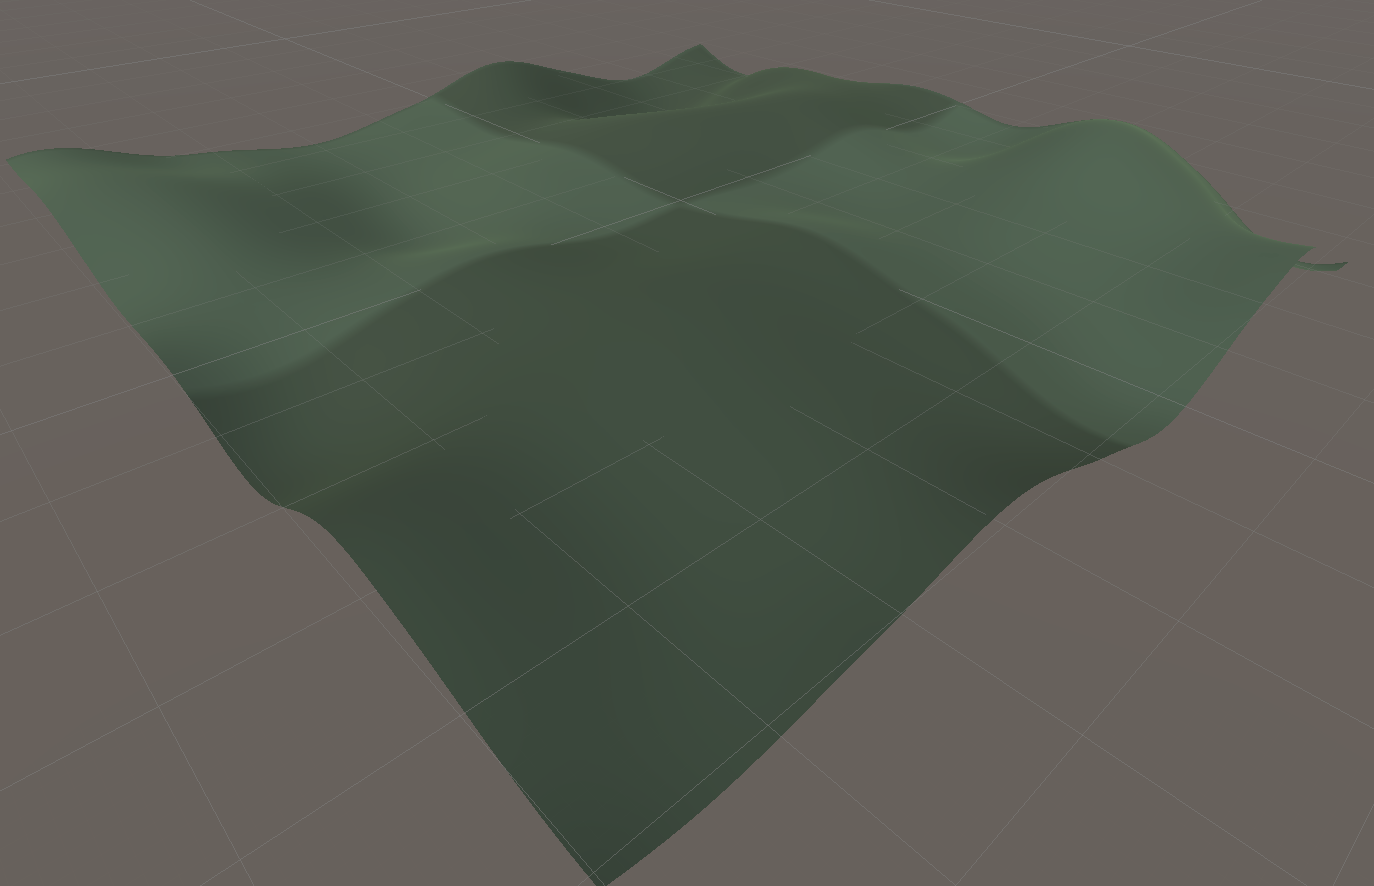
\includegraphics[width=\linewidth]{lacunarity1.png}
        \caption{$l=1$}
        \label{fig:lacunarity1}
    \end{subfigure}
    \hfill
    \begin{subfigure}{0.3\textwidth}
        \centering
        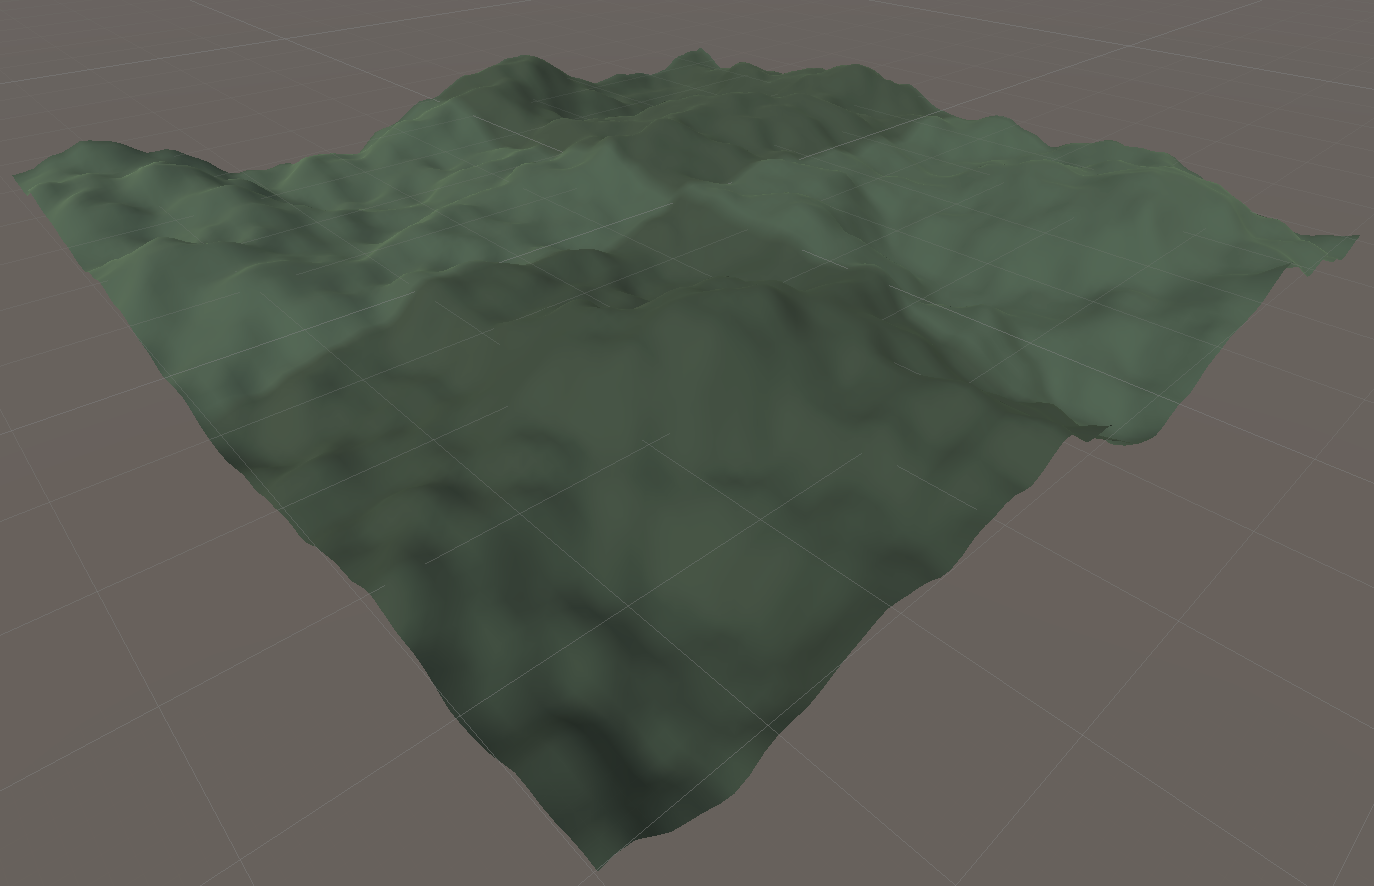
\includegraphics[width=\linewidth]{lacunarity2.png}
        \caption{$l=2$}
        \label{fig:lacunarity2}
    \end{subfigure}
    \hfill
    \begin{subfigure}{0.3\textwidth}
        \centering
        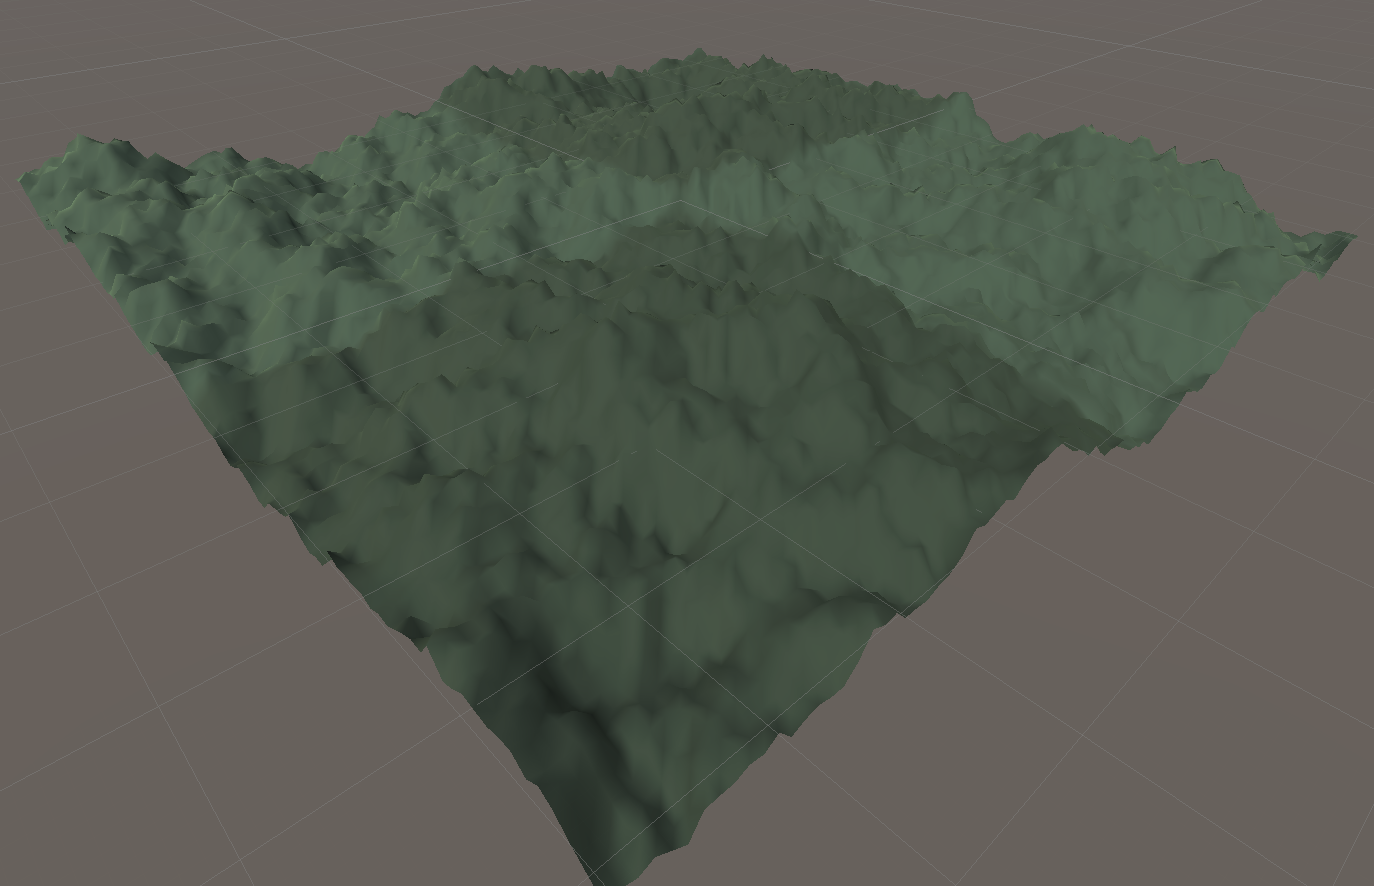
\includegraphics[width=\linewidth]{lacunarity4.png}
        \caption{$l=4$}
        \label{fig:lacunarity4}
    \end{subfigure}
    \caption{The effect of lacunarity on the generated terrain}
    \label{fig:lacunarity}
\end{figure}


The persistence, $p$, controls the decrease in amplitude between octaves. This allows us to tune how much each subsequent octave decreases in contribution to the overall waveform. This is characterised by the relationship:

$$\forall x \in \{O_1,O_2,...,O_n\}, A_x = p^{O_x}$$

We can see below, in Fig. \ref{fig:persistence}, the effect of persistence on the generated terrain. We can see that as the persistence increases, the height of the smaller details in the terrain increases. As we have kept the lacunarity constant, the spikes are not as evident as with Fig. \ref{fig:lacunarity4}.

\begin{figure}[H]
    \centering
    \begin{subfigure}{0.3\textwidth}
        \centering
        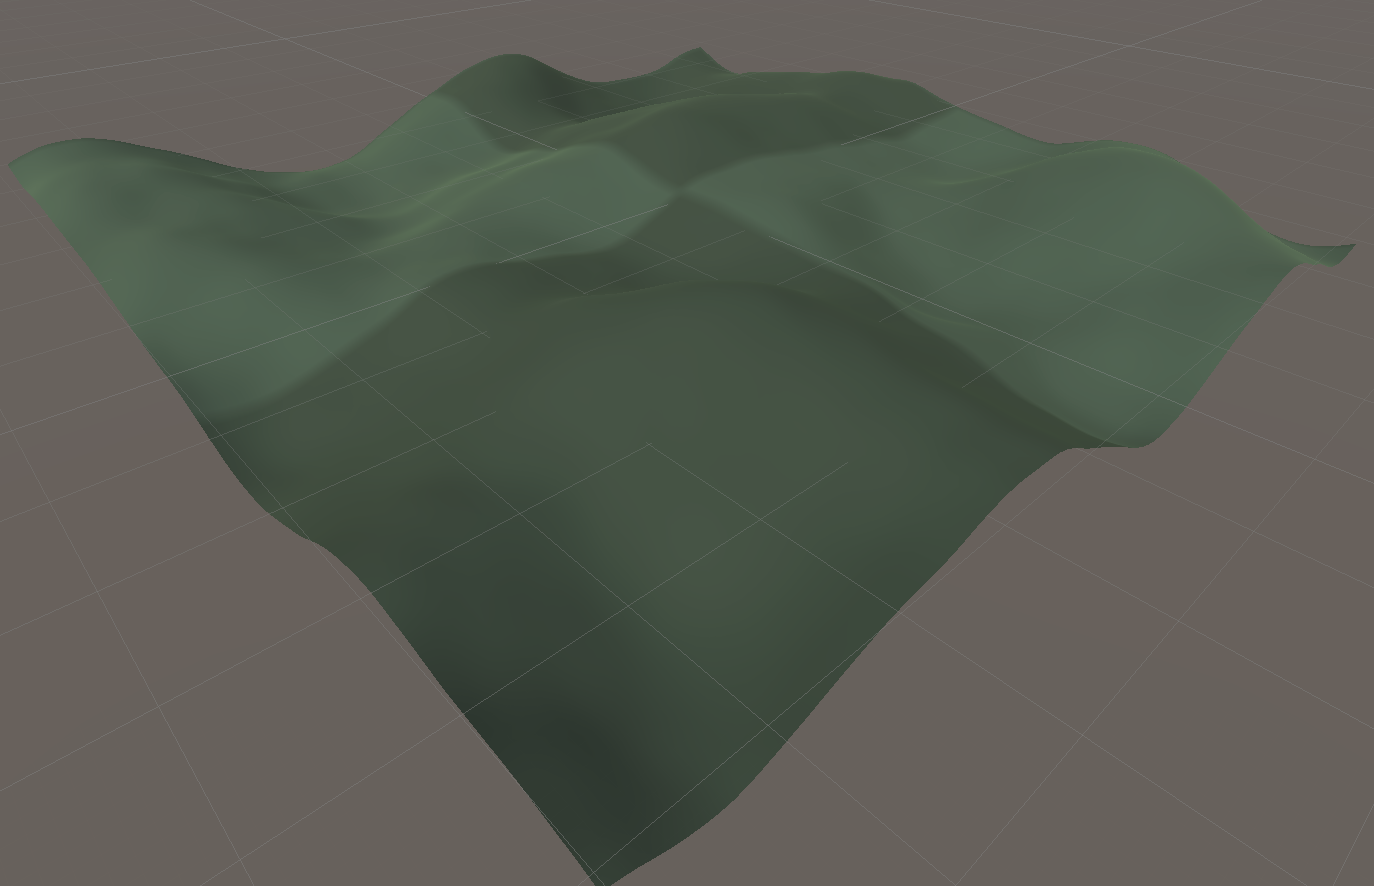
\includegraphics[width=\linewidth]{persistance0.2.png}
        \caption{$p=0.2$}
        \label{fig:persistence0.2}
    \end{subfigure}
    \hfill
    \begin{subfigure}{0.3\textwidth}
        \centering
        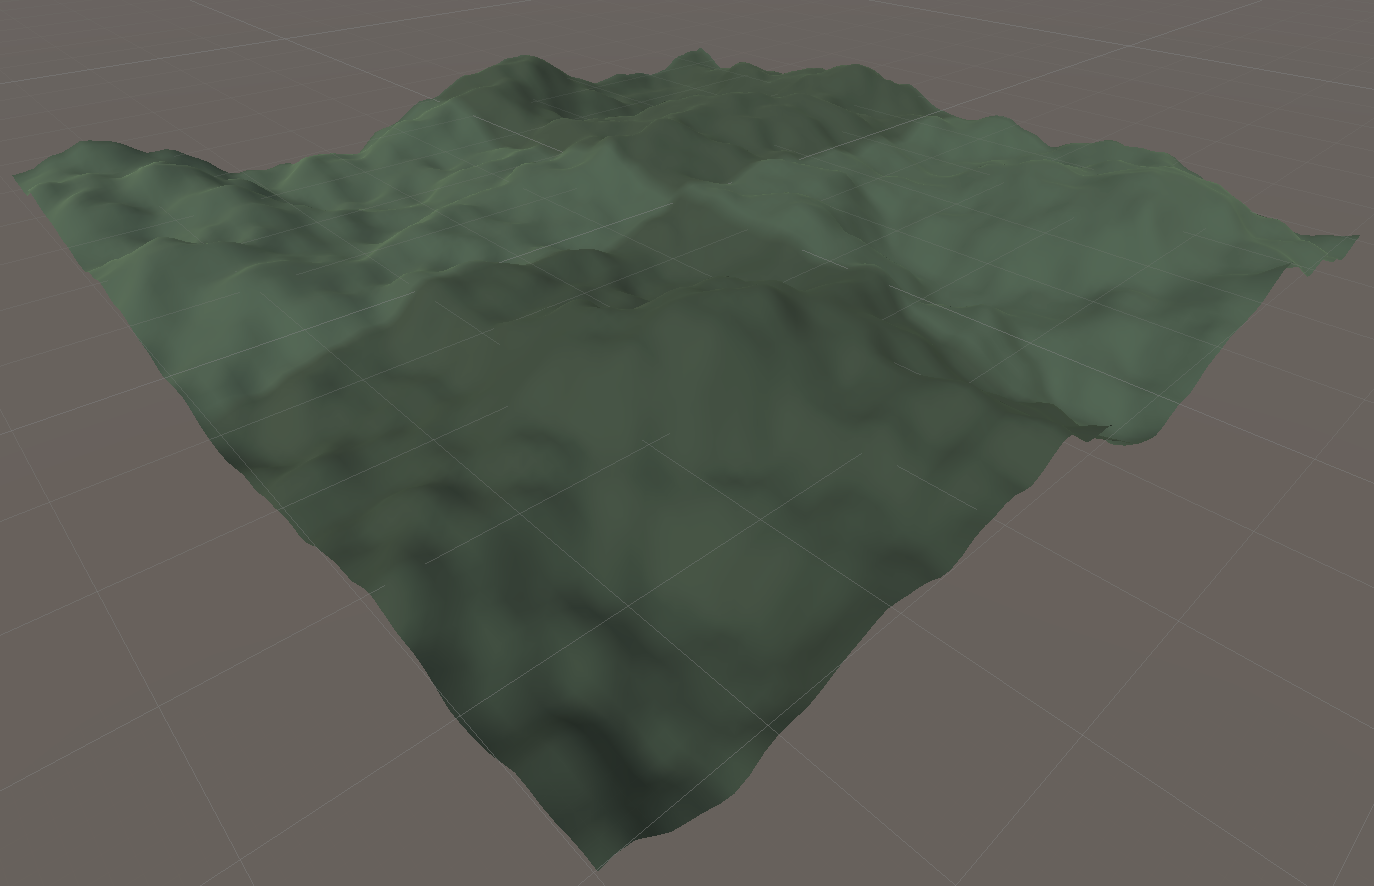
\includegraphics[width=\linewidth]{persistance0.5.png}
        \caption{$p=0.5$}
        \label{fig:persistence0.5}
    \end{subfigure}
    \hfill
    \begin{subfigure}{0.3\textwidth}
        \centering
        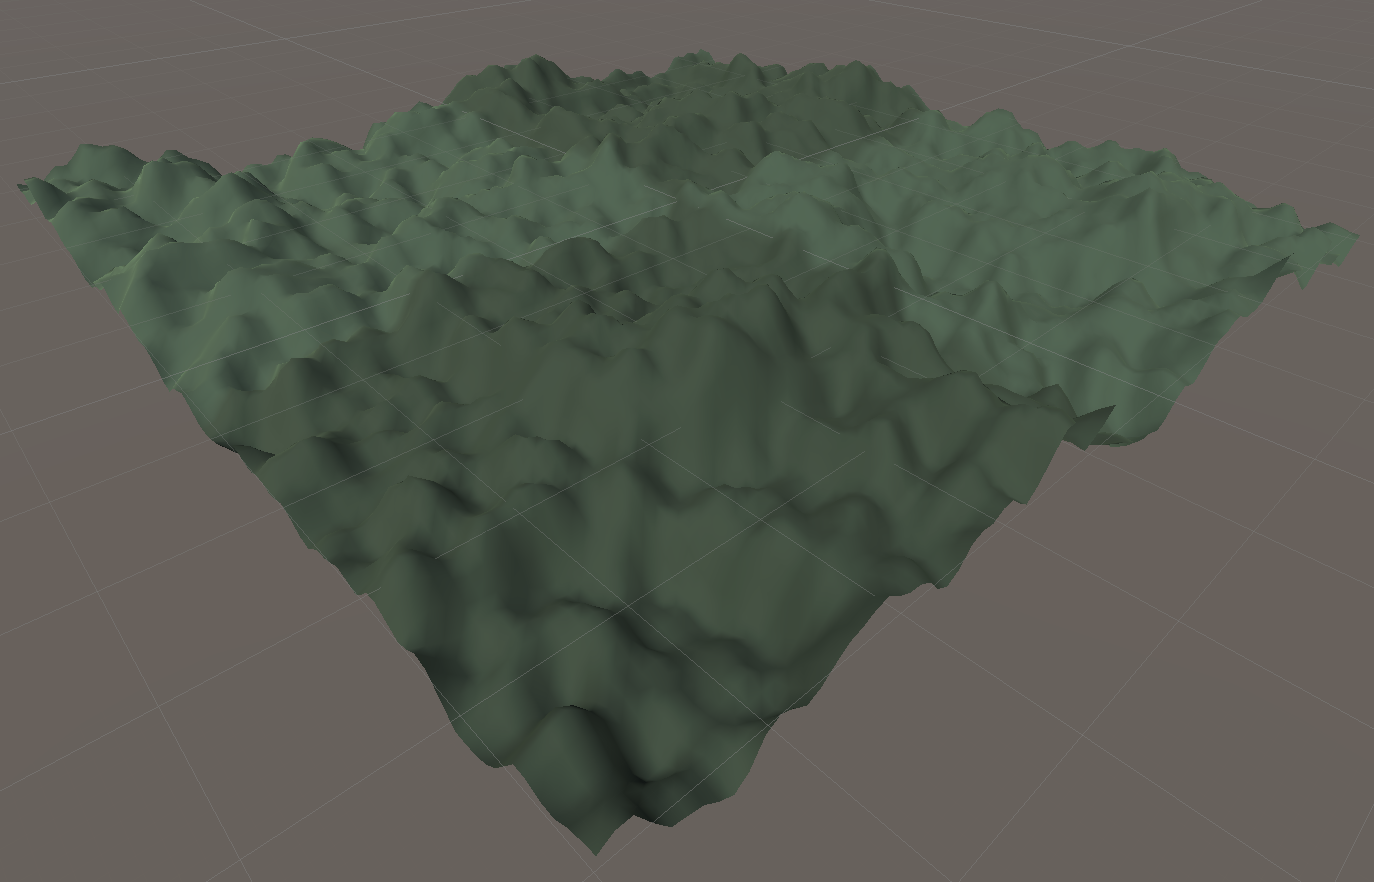
\includegraphics[width=\linewidth]{persistance0.8.png}
        \caption{$p=0.8$}
        \label{fig:persistence0.8}
    \end{subfigure}
    \caption{The effect of persistence on the generated terrain}
    \label{fig:persistence}
\end{figure}

Finally, the scale, $s$, contols the level of detail in the waveform that is applied to the terrain. We see in Fig. \ref{fig:scale}, the effect of scale on the generated terrain. We can see that as the scale increases, the terrain becomes more `zoomed out', and the details become less prominent. Notably, we can see a mountain ridge in the quadrant closest to the camera increase in size and distance away from the origin\footnote{The origin is the top left (the quadrant furthest away from the camera) of the terrain mesh.} between Fig. \ref{fig:scale25} and Fig. \ref{fig:scale28}.

\begin{figure}[H]
    \centering
    \begin{subfigure}{0.45\textwidth}
        \centering
        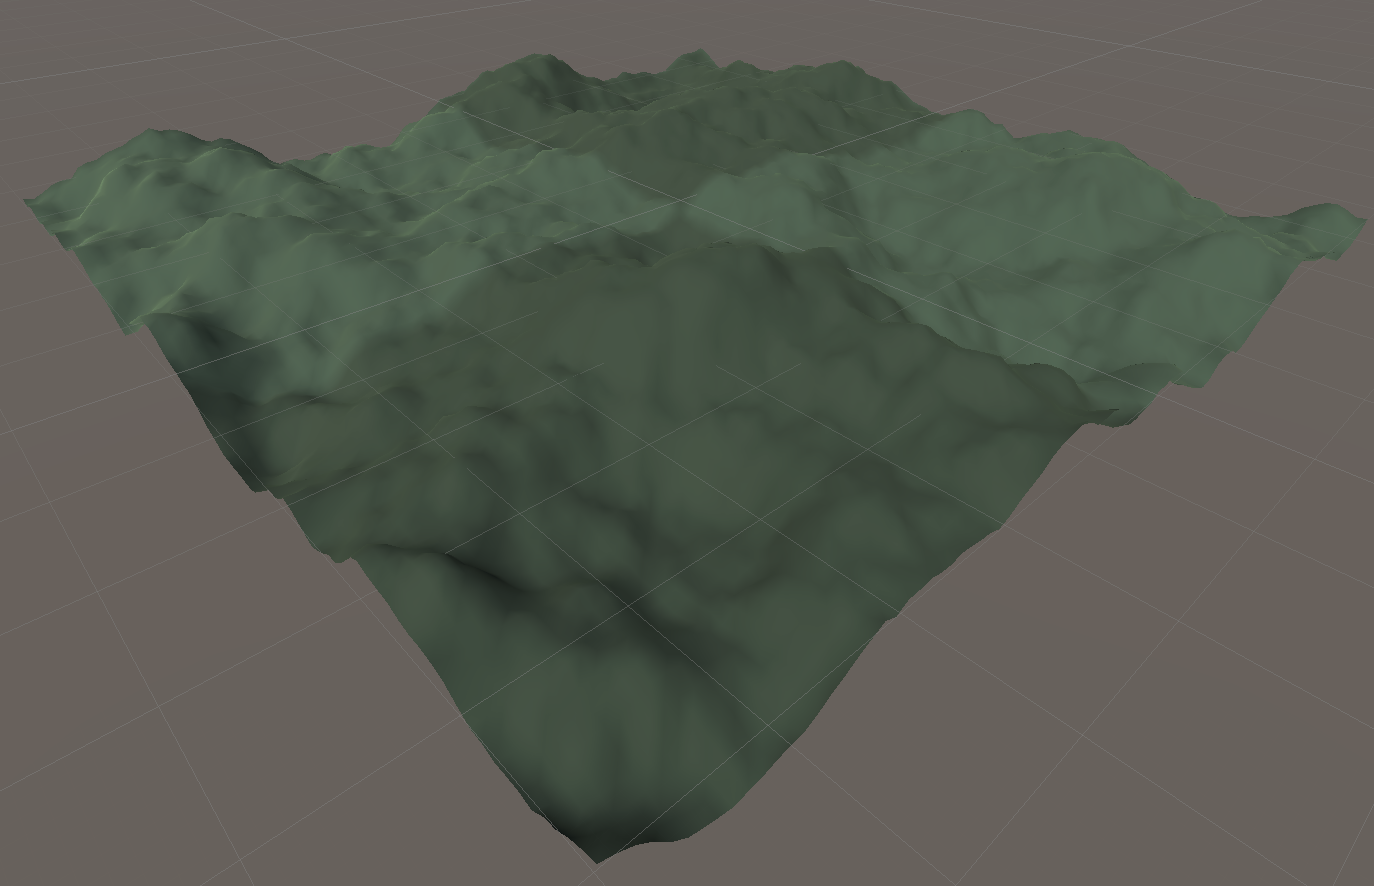
\includegraphics[width=\linewidth]{scale25.png}
        \caption{$s=25$}
        \label{fig:scale25}
    \end{subfigure}
    \hfill
    \begin{subfigure}{0.45\textwidth}
        \centering
        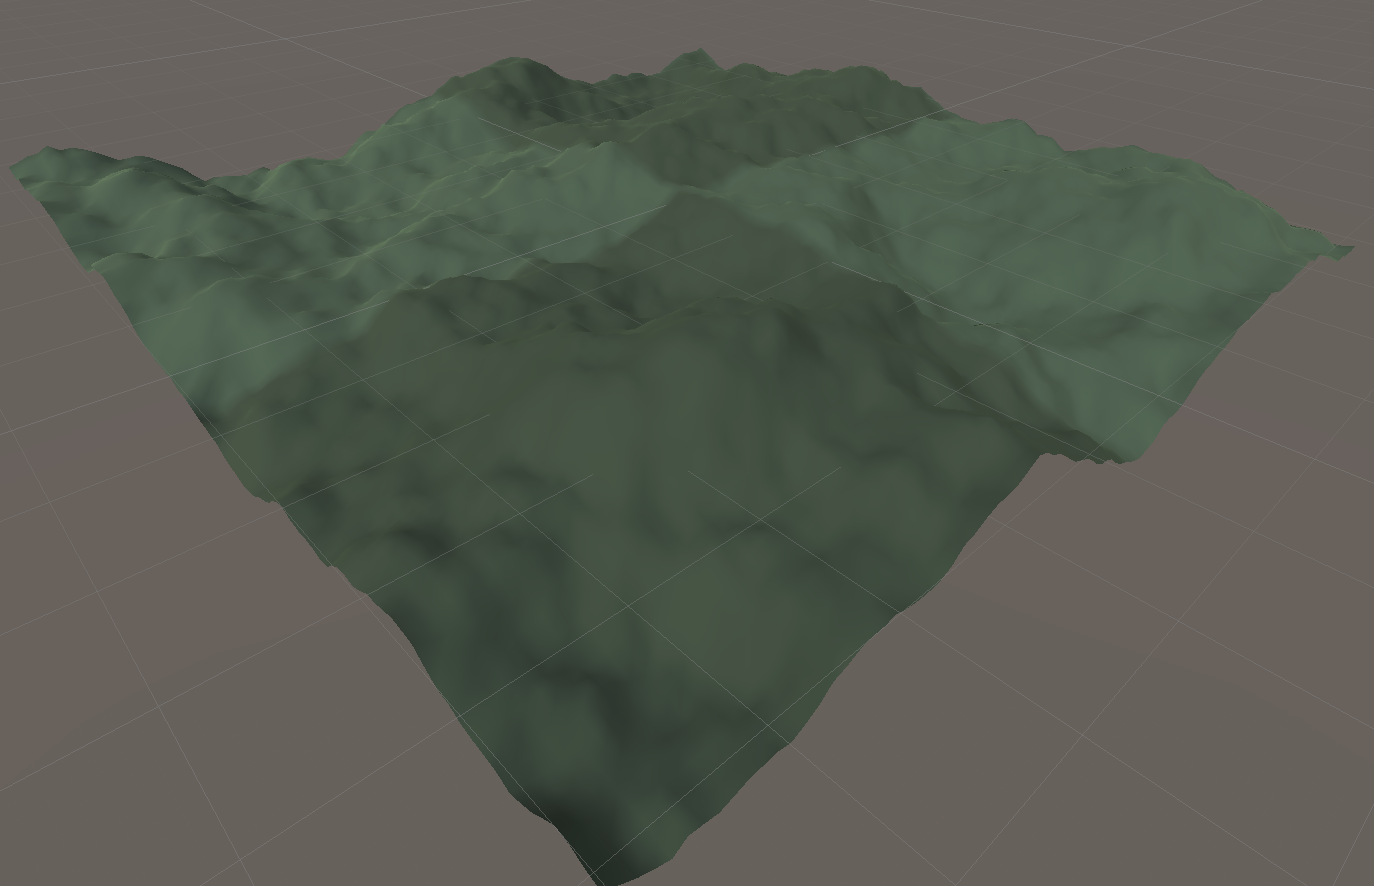
\includegraphics[width=\linewidth]{scale28.png}
        \caption{$s=28$}
        \label{fig:scale28}
    \end{subfigure}
    \caption{The effect of scale on the generated terrain}
    \label{fig:scale}
\end{figure}

After tuning the parameters based on a combination of empirical methods and noted examples \cite[pg.3-4]{Etherington}, the following parameters were chosen, with the final terrain mesh shown alongside:

\begin{figure}[ht]
    \centering
    \begin{subfigure}{0.4\textwidth}
        \centering
        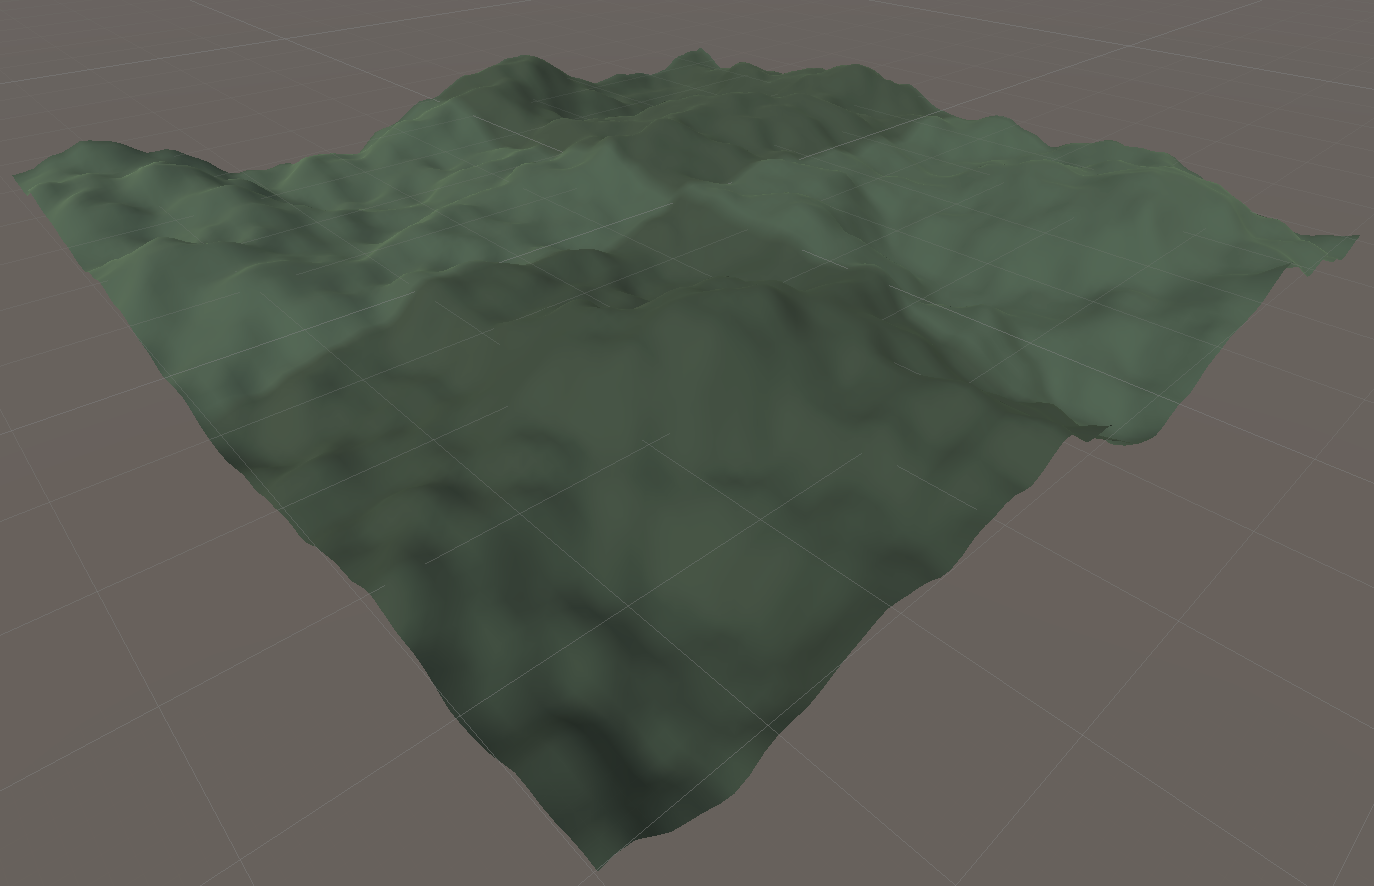
\includegraphics[width=\linewidth]{lacunarity2.png}
        \caption{Final Terrain Mesh}
        \label{fig:final}
    \end{subfigure}
    \hfill
    \begin{subfigure}{0.4\textwidth}
        \centering
        \begin{tabular}{|c|c|}
            \hline
            Number of Octaves & 4 \\
            \hline
            Parameter & Value \\
            \hline
            Lacunarity & 2 \\
            \hline
            Persistence & 0.5 \\
            \hline
            Scale & 25 \\
            \hline
        \end{tabular}
        \caption{Perlin Noise Parameter Values}
        \label{tab:parameter-values}
    \end{subfigure}
    \caption{}
    \label{fig:parameter-values-lacunarity2}
\end{figure}

\subsection{Terrain Avoidance}
\label{sec:terrain-avoidance}
\subsubsection{A Naive Model}
Earlier, in Section \ref{sec:vision}, we introduced the agents' ability to determine range from a light ranging sensor, or LiDAR. We can use this to determine the distance between the agent and the terrain mesh. Initially, we will model the sensor as a single point on the bottom of the agent, which casts a singular light ray downwards.

We can then perform terrain avoidance by generating upward thrust to cause an increase in the agent's $y$ position if the distance between the agent and the terrain is less than a given threshold. We will initially set this threshold to 5 metres.

We can see this behaviour in operation in Fig. \ref{fig:naive-ta-1}, where an agent approaches a steep hill. We see that before point 1, the agent does not increase its altitude. When a ray is cast at point 1, the agent detects that the distance between itself and the terrain is less than the threshold, and increases its altitude. Point 2 is the crest of the hill. At this point, the agent detects that there is still not enough distance between itself and the terrain, so the altitude continues to increase. In Fig. \ref{fig:naive-ta-2}, we see that the agent has detected the terrain, but appears to carry too much forward momentum and is locked in a tilt, so cannot avoid the hill.

\begin{figure}[H]
    \centering
    \begin{subfigure}{0.45\textwidth}
        \centering
        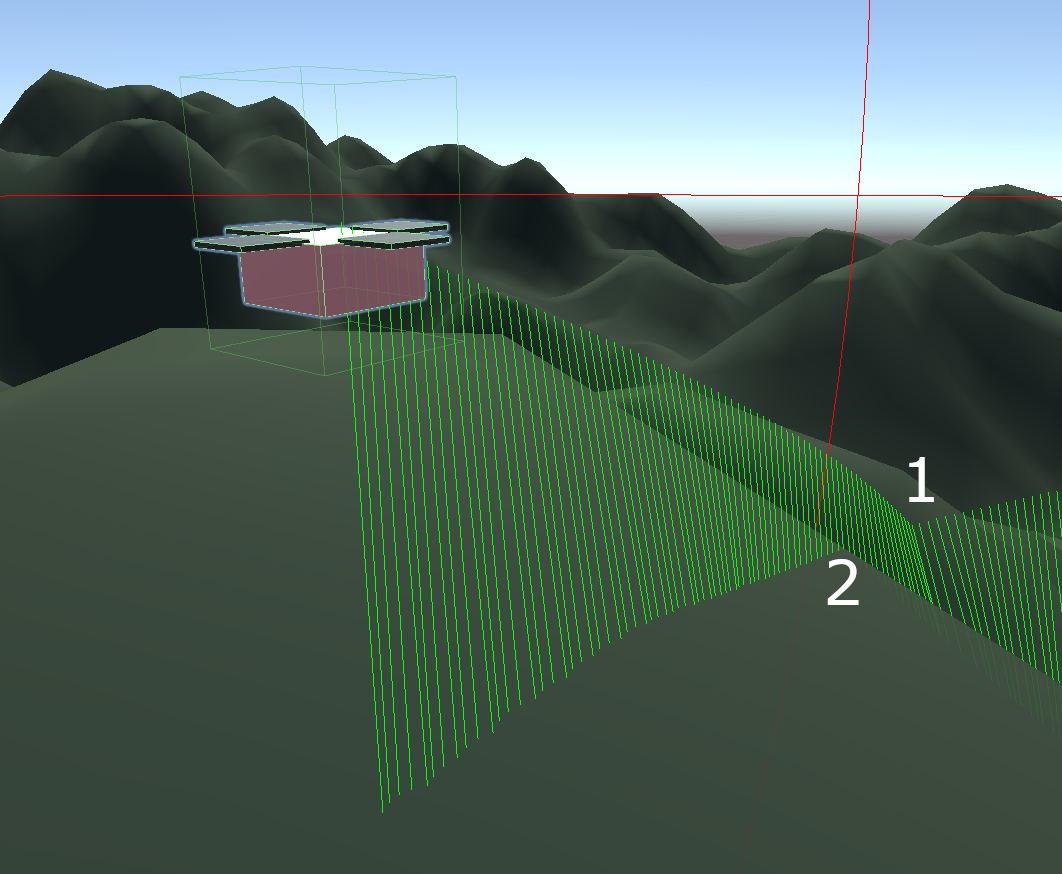
\includegraphics[width=\linewidth]{naive-ta-edited.png}
        \caption{Agent approaching a steep hill}
        \label{fig:naive-ta-1}
    \end{subfigure}
    \hfill
    \begin{subfigure}{0.45\textwidth}
        \centering
        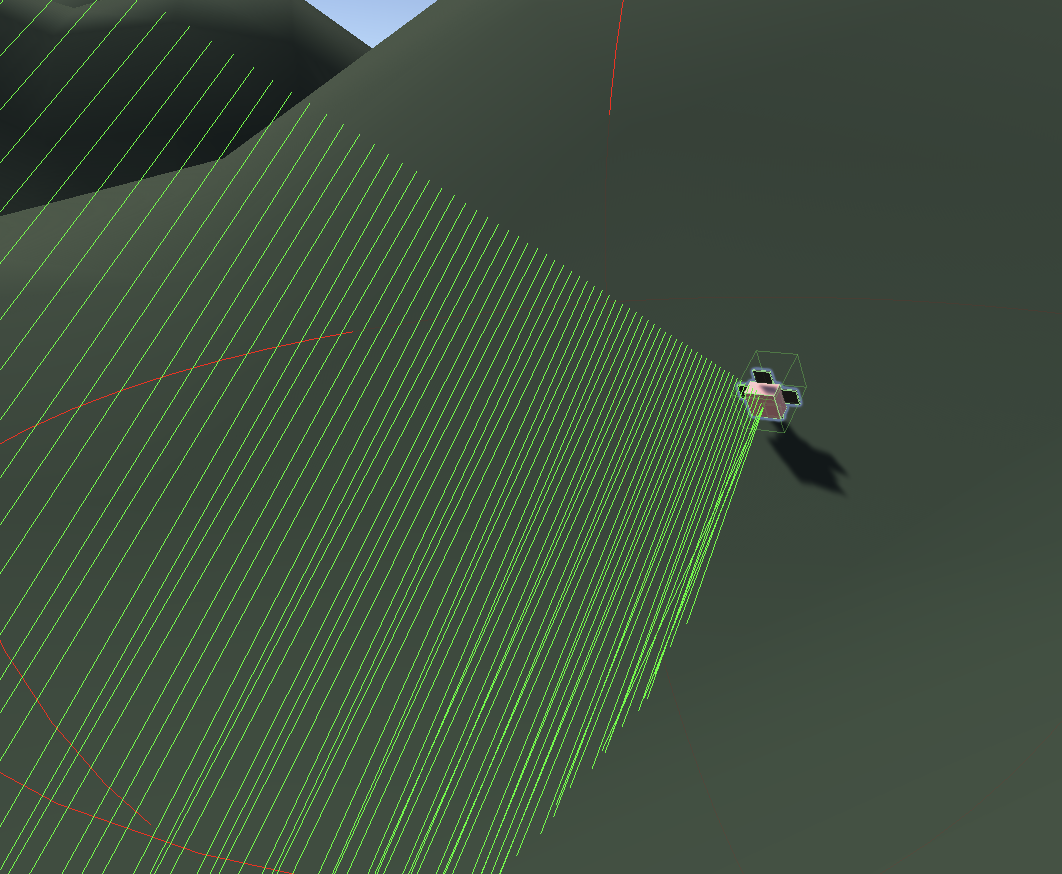
\includegraphics[width=\linewidth]{naive-ta-2.png}
        \caption{Agent failing to avoid terrain}
        \label{fig:naive-ta-2}
    \end{subfigure}
    \caption{Naive Terrain Avoidance}
    \label{fig:naive-ta-side-by-side}
\end{figure}

These two observations reveal two important modifications that need to be made to our avoidance system:
\begin{enumerate}
    \item The agent needs to be able to detect the terrain in front of it, not just below it.
    \item The agent needs to be able to detect the terrain at a greater distance.
\end{enumerate}

\subsubsection{Improving The Model}
\label{sec:improving-the-model}
To address our concerns, we can adjust the angle of the LiDAR scanner along the pitch axis of the agent to face slightly forward. This should allow the agent to detect the terrain in front of it, as well as below it. We will also increase the avoidance range of the agent to 10 meters to counter steeper hills. 

Unfortunately, the scale of the terrain proved a large challenge in optimising the avoidance behaviour.

\subsection{Tuning the Boids Model}
In line with the terrain changes, we will make some changes to how the simulation begins and ends. We define two platforms - a (red) start platform and a (green) end platform. The start platform is a flat surface, with a radius of 4, centred at the origin. The end platform is a flat surface, with a radius of 4, centred at a random point within a radius of 100m of the origin. The agents will begin on the start platform, and will be instructed to seek the end platform. These platforms are seen below in Fig. \ref{fig:platforms}.

\begin{figure}[H]
    \centering
    \begin{subfigure}{0.45\textwidth}
        \centering
        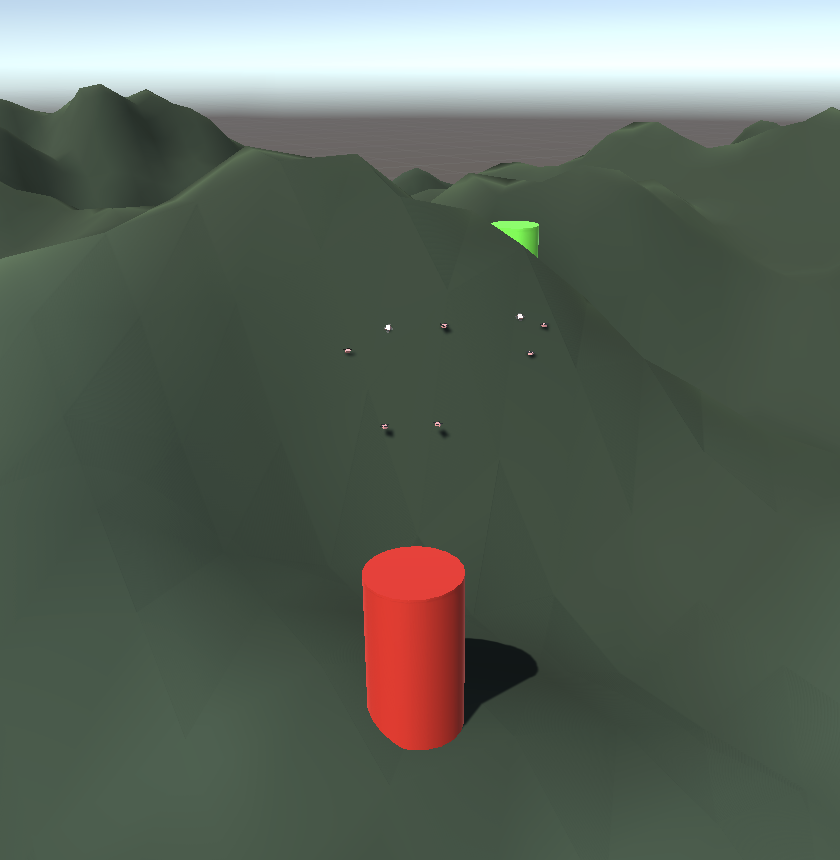
\includegraphics[width=\linewidth]{startplatform.png}
        \caption{Start Platform}
        \label{fig:startplatform}
    \end{subfigure}
    \hfill
    \begin{subfigure}{0.45\textwidth}
        \centering
        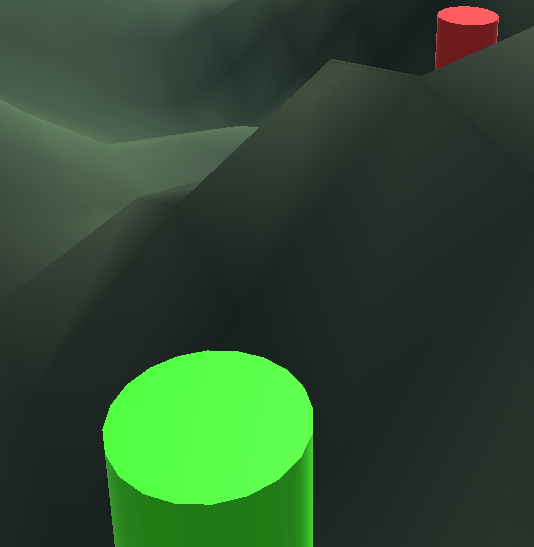
\includegraphics[width=\linewidth]{goalplatform.png}
        \caption{Goal Platform}
        \label{fig:goalplatform}
    \end{subfigure}
    \caption{Start and Goal Platforms in a single simulation}
    \label{fig:platforms}
\end{figure}



% \section{Complex Pathfinding for Hostile Environments}
% \label{sec:complex-pathfinding}
% \subsection{A* - The Hacks \& Bodges?}

% \subsection{Pair Potential Model}

% \subsubsection{Obstacle Avoidance}

\section{Real World Limitations}
\subsection{Real World Represenation}

\subsection{Sensing \& Vision}

\section{Extensions}
\subsection{Obstacle Detection}

\subsection{Semi-Autonomous Control}

\section{Evaluation}
\subsection{Speed-Success-Flock Size Tradeoffs}

\subsection{Use Cases}




\newpage
\bibliographystyle{IEEEtran}
\bibliography{refs} 
\end{document}

